\documentclass[reprint,english,notitlepage]{revtex4-2}  % defines the basic parameters of the document

% if you want a single-column, remove reprint

% allows special characters (including æøå)
\usepackage[utf8]{inputenc}
\usepackage[english]{babel}

%% note that you may need to download some of these packages manually, it depends on your setup.
%% I recommend downloading TeXMaker, because it includes a large library of the most common packages.

\usepackage{physics,amssymb}  % mathematical symbols (physics imports amsmath)
\usepackage{graphicx}         % include graphics such as plots
\graphicspath{ {./Figures/} }
\usepackage{xcolor}           % set colors
\usepackage{hyperref}         % automagic cross-referencing (this is GODLIKE)
\usepackage{tikz}             % draw figures manually
\usepackage{listings}         % display code
\usepackage{subfigure}        % imports a lot of cool and useful figure commands
\usepackage[section]{placeins}

% defines the color of hyperref objects
% Blending two colors:  blue!80!black  =  80% blue and 20% black
\hypersetup{ % this is just my personal choice, feel free to change things
    colorlinks,
    linkcolor={red!50!black},
    citecolor={blue!50!black},
    urlcolor={blue!80!black}}

%% Defines the style of the programming listing
%% This is actually my personal template, go ahead and change stuff if you want
\lstset{ %
	inputpath=,
	backgroundcolor=\color{white!88!black},
	basicstyle={\ttfamily\scriptsize},
	commentstyle=\color{magenta},
	language=Python,
	morekeywords={True,False},
	tabsize=4,
	stringstyle=\color{green!55!black},
	frame=single,
	keywordstyle=\color{blue},
	showstringspaces=false,
	columns=fullflexible,
	keepspaces=true}


%% USEFUL LINKS:
%%
%%   UiO LaTeX guides:        https://www.mn.uio.no/ifi/tjenester/it/hjelp/latex/ 
%%   mathematics:             https://en.wikibooks.org/wiki/LaTeX/Mathematics

%%   PHYSICS !                https://mirror.hmc.edu/ctan/macros/latex/contrib/physics/physics.pdf

%%   the basics of Tikz:       https://en.wikibooks.org/wiki/LaTeX/PGF/TikZ
%%   all the colors!:          https://en.wikibooks.org/wiki/LaTeX/Colors
%%   how to draw tables:       https://en.wikibooks.org/wiki/LaTeX/Tables
%%   code listing styles:      https://en.wikibooks.org/wiki/LaTeX/Source_Code_Listings
%%   \includegraphics          https://en.wikibooks.org/wiki/LaTeX/Importing_Graphics
%%   learn more about figures  https://en.wikibooks.org/wiki/LaTeX/Floats,_Figures_and_Captions
%%   automagic bibliography:   https://en.wikibooks.org/wiki/LaTeX/Bibliography_Management  (this one is kinda difficult the first time)
%%   REVTeX Guide:             http://www.physics.csbsju.edu/370/papers/Journal_Style_Manuals/auguide4-1.pdf
%%
%%   (this document is of class "revtex4-1", the REVTeX Guide explains how the class works)


%% CREATING THE .pdf FILE USING LINUX IN THE TERMINAL
%% 
%% [terminal]$ pdflatex template.tex
%%
%% Run the command twice, always.
%% If you want to use \footnote, you need to run these commands (IN THIS SPECIFIC ORDER)
%% 
%% [terminal]$ pdflatex template.tex
%% [terminal]$ bibtex template
%% [terminal]$ pdflatex template.tex
%% [terminal]$ pdflatex template.tex
%%
%% Don't ask me why, I don't know.

\begin{document}
\title{FYS-STK3155 - Project 2}   % self-explanatory
\author{Dag Arne Lydvo}               % self-explanatory
\date{\today}                             % self-explanatory
\noaffiliation                            % ignore this
\begin{abstract}                          % marks the beginning of the abstract
In this project I will be writing a neural network class to employ at both regression and classification tasks. The network will be compared with both linear regression with and without regularization including a Scikit-learn neural net. Neural networks as proves to be stable on regression tasks and avoids over fitting, this is also true for the Ridge regression. On the classification task the neural networks performs very well, but are dependent on the learning rate and not so much the regularization parameter, this seems to change when adding more layers. 
\end{abstract}                            % marks the end of the abstract
\maketitle                                % creates the title, author, date & abstract


% the fundamental components of scientific reports:
\section{Introduction}
This project seeks to utilize neural networks to perform both regression and classification tasks. For the regression section I will be revisiting the Franke function from project 1 and employ a neural network as well as linear regression methods and do a comparison. 

In the classification section the neural network will be employed to classify handwritten numbers from the MNIST dataset. I will be looking at different learning rates, regularization parameters and different number of hidden layers in the network. A neural network from Scikit-learn will also be implemented for comparison. 


\section{Method}
\subsection{Stochastic gradient descent}
The stochastic gradient descent is implemented to improve training speed versus the normal gradient descent which uses the whole training set and can be quite computational expensive. 
Gradient descent method seeks to minimize a cost function by finding the fastest way to a minimum, preferably a global minimum. The method seeks to reach the point where the gradient of the cost function is zero by iteration tweaking parameters of a model until a minimum is found. In the equation below theta represents the various parameters of a model and gamma is a learning rate. [1]

\[ \theta^{next step} = \theta - \gamma \grad_{\theta}MSE(\theta) \] 

The stochastic gradient descent picks random instances of the training sets and uses the sample to compute the gradient. The SGD is much more irregular than ordinary gradient descent. This can be an advantage when trying to avoid getting stuck in local minima. 

\subsection{Neural networks}
Neural networks are ordered in layers with various number of nodes. 
A network got an input layer corresponding to the number of features in the design matrix. Then a number of hidden layers before the output layer with number of nodes corresponding to the number of output values.
The nodes in the hidden layers are activated by a activation function which is a sum of the input values from the previous layer multiplied by weights corresponding to each connection then a bias term is added, the bias belongs to a a specific node while the biases to every connection to a node.

\[ z = \omega^la^{l-1} + b^l\]Node input 
\[ a^l(z) = \sigma(z)\] Activation function
\begin{figure}[!ht]
	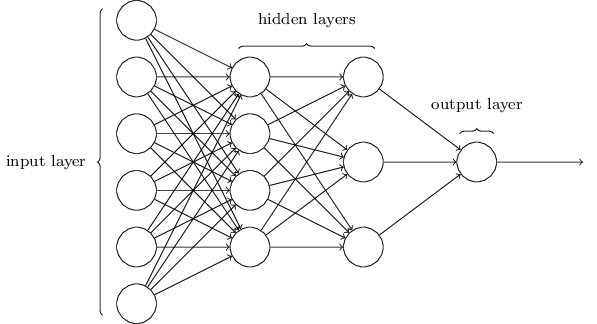
\includegraphics[scale=0.25]{neuralnetarch}
\end{figure}

\subsection{Accuracy score}
For classification an accuracy score is used 
\[ Accuracy = \frac{\sum_{i=1}^{n}I(t_i=y_i)}{n}\]
The accuracy scores measure the number of successful classifications over the number of data points being classified. The function I here produces 1 if classification is successful otherwise 0. 
\subsection{Regression methods}
For regression in this project in addition to a neural network I will be using the Linear regression and Ridge regression specified in project 1. 

\subsection{Datasets}
\subsubsection{The Franke function}
For the regression part of this project I will be using the Franke function used and described in project 1. 

\subsubsection{MNIST digits dataset}
For classification the MNSIT dataset of handwritten numbers will be used. 
\begin{figure}[!htb]
	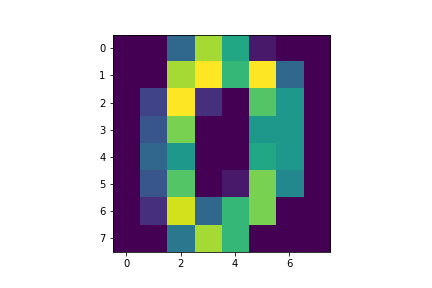
\includegraphics[trim=140 20 0 0, scale=0.4]{MNIST figure 1}
	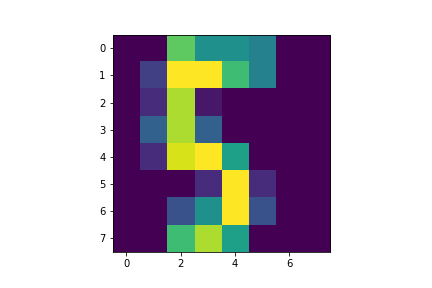
\includegraphics[trim=140 20 0 0, scale=0.4]{MNIST figure 2}
	\caption{Examples of 8x8 pixels pictures of handwritten figures of the MNIST dataset.}\label{figure}
	
The dataset is imported using the Scikit-learn library and module datasets.
There are a total of 1797 numbers, each with 8x8 pixels giving a total of 64 features.  
\end{figure}





\newpage


\section{Results}
Running an experiment with linear regression with and without regularization using stochastic gradient descent over the Franke function, using the Scikit-learn SGD module for comparison. 
\begin{figure}[!htb]
	\centering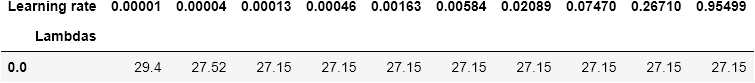
\includegraphics[trim=140 20 100 0, scale=0.4]{OLSSGD}
	\caption{Mean squared error score for Linear regression using SGD }\label{figure}
\end{figure}
\begin{figure}[!htb]
	\centering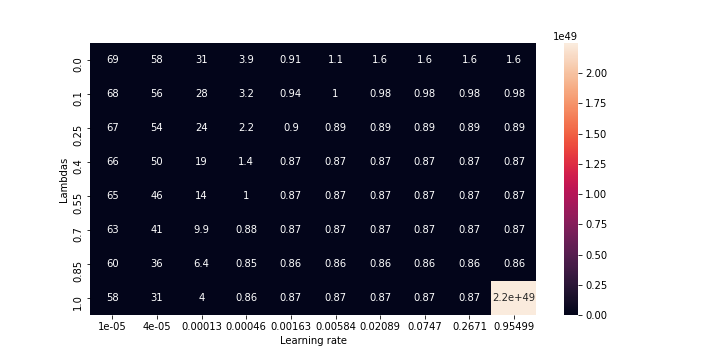
\includegraphics[trim=75 10 0 0, scale=0.45]{SGD Ridge}
	\caption{Mean squared error score for Ridge regression using SGD }\label{figure}
\end{figure}
\begin{figure}[!htb]
	\centering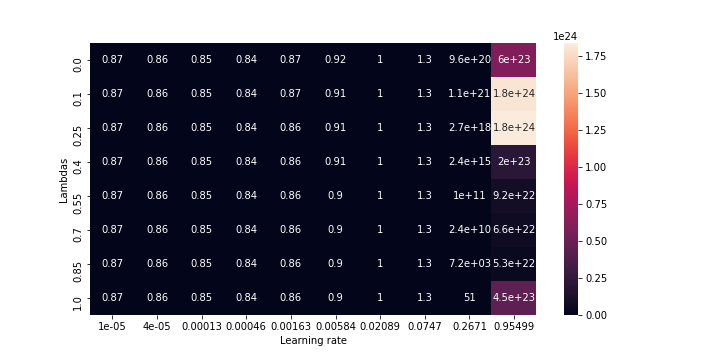
\includegraphics[trim=75 10 0 70, scale=0.45]{SGD Sklearn OLS}
	\caption{Mean squared error score for SGD Regression using Sklearn with regularization parameter lambda, $\lambda$. }\label{figure}
	\end{figure}

Results for regression experiments on the Franke function using a neural network. 

\begin{figure}[!htb]
	\centering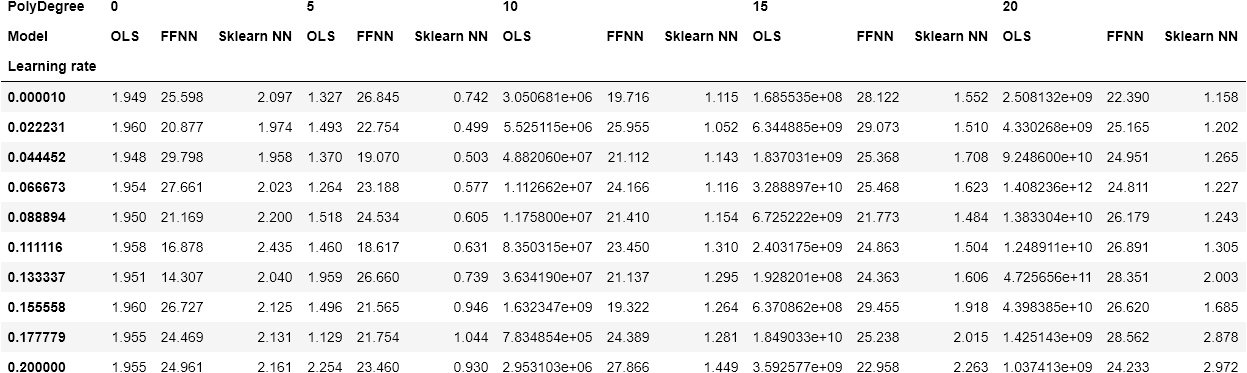
\includegraphics[trim=75 20 100 0, scale=0.30]{Partb-1}
	\caption{Mean squared error score for 3 models, OLS, a neural net class and a Scikit-learn neural net over selected model complexities (Polynomial degree) and different learning rates.  }\label{figure}
\end{figure}
\begin{figure}[!htb]
	\centering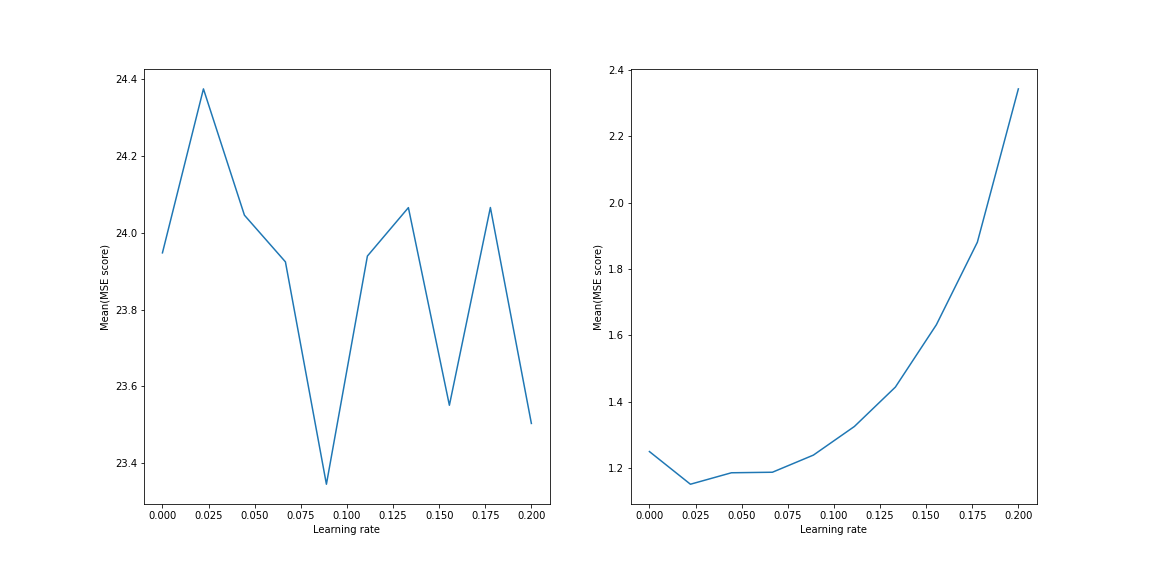
\includegraphics[trim=75 20 0 0, scale=0.25]{Partb-2}
	\caption{The Mean of the MSE score for all polynomial degrees for the NN class and the Scikit-learn NN, ploted against the range of learning rates.}\label{figure}
\end{figure}

Tests using learning rate of 0.1 
\begin{figure}[!htb]
	\centering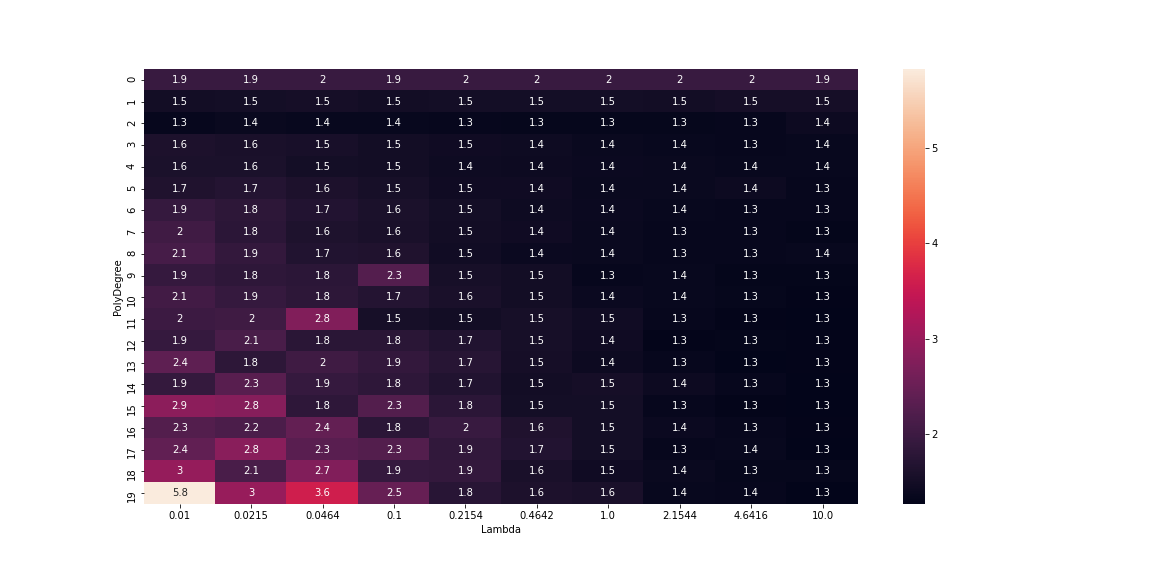
\includegraphics[trim=75 20 0 0, scale=0.3]{Partb-3}
	\caption{Mean squared error scores for Ridge regression over values of Lambda and Polynomial degrees. }\label{figure}
\end{figure}
\begin{figure}[!htb]
	\centering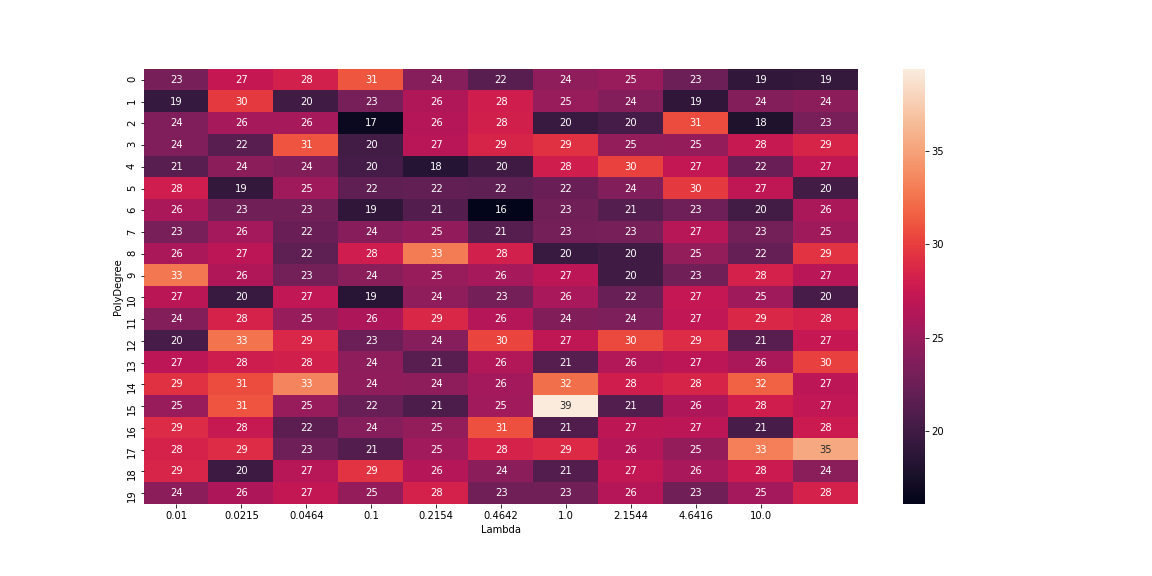
\includegraphics[trim=75 20 0 0, scale=0.3]{Partb-4}
	\caption{Mean squared error scores for Neural network regression over values of Lambda and Polynomial degrees.}\label{figure}
\end{figure}
\begin{figure}[!htb]
	\centering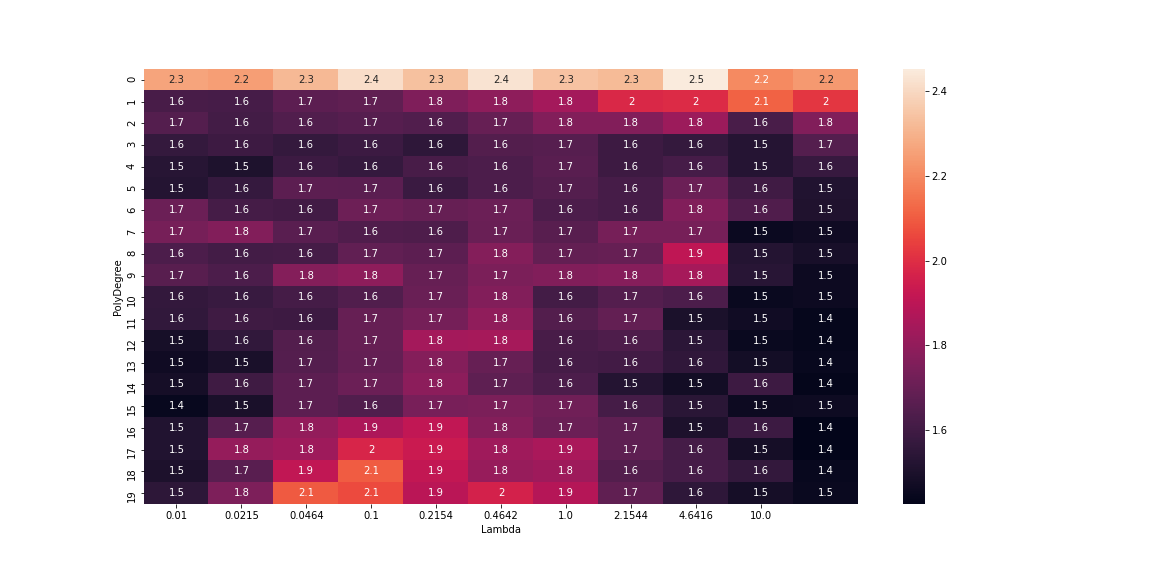
\includegraphics[trim=75 20 0 200, scale=0.3]{Partb-5}
	\caption{Mean squared error scores for the Scikit-learn Neural network regression over values of Lambda and Polynomial degrees}\label{figure}
\end{figure}
\begin{figure}[!htb]
	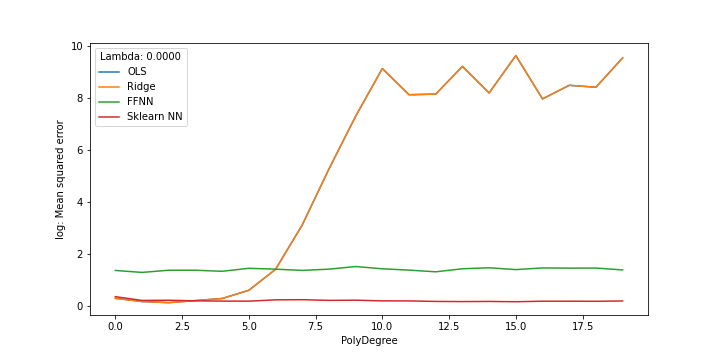
\includegraphics[trim=75 70 0 0, scale=0.3]{NNReg1}
	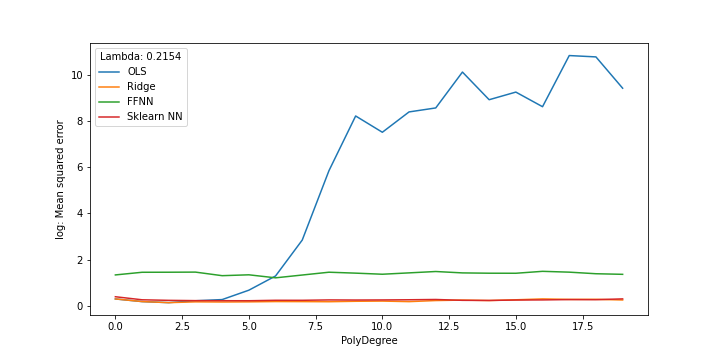
\includegraphics[trim=75 70 0 0, scale=0.3]{NNReg2}
	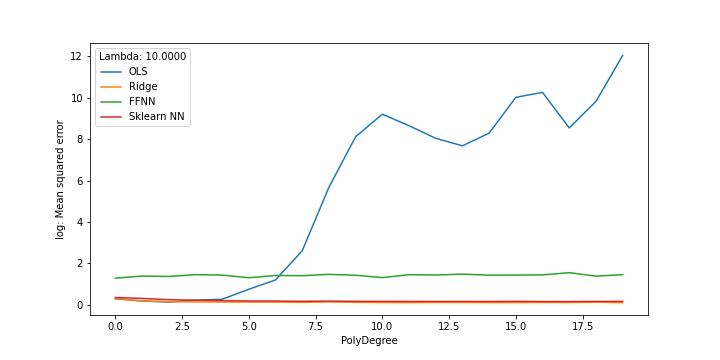
\includegraphics[trim=75 50 0 0, scale=0.3]{NNReg3}
	\caption{Mean squared error scores for all four models over Polynomial degree, plottet at selected values of lambda. }\label{figure}
	
\end{figure}

Testing of different activation functions.
\begin{figure}[!htb]
	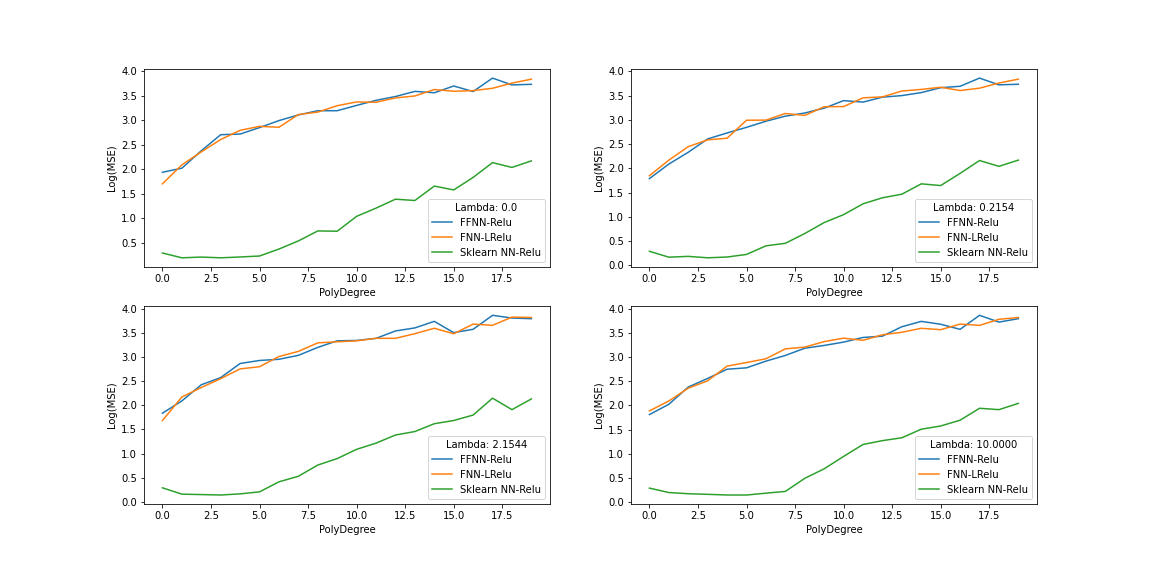
\includegraphics[trim=75 70 0 0, scale=0.25]{Partc-1}
	\caption{Log(MSE) for neural network implementation using RELU and leaky RELU activation functions for the hidden layer over polynomial degrees.   }\label{figure}
	
\end{figure}
\begin{figure}[!htb]
	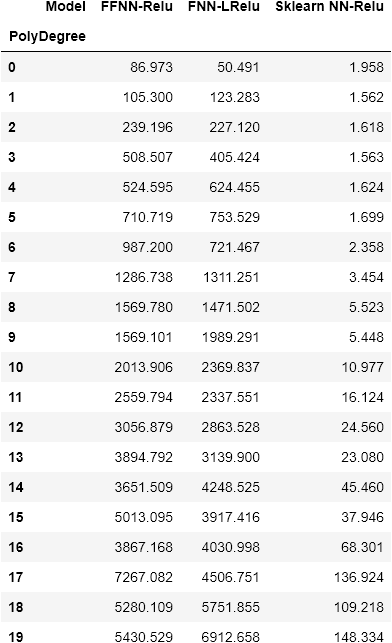
\includegraphics[trim=75 0 0 0, scale=0.4]{Partc-2}
	\caption{MSE score for RELU and leaky RELU implementation of my neural network at $lambda=0$. RELU activation for the Scikit-learn  implementation.    }\label{figure}
	
\end{figure}


\section{Classification results}
\begin{text}
	
	The following are results from classification experiments on the MNIST dataset...
\end{text}
 

\begin{figure}[!htb]
	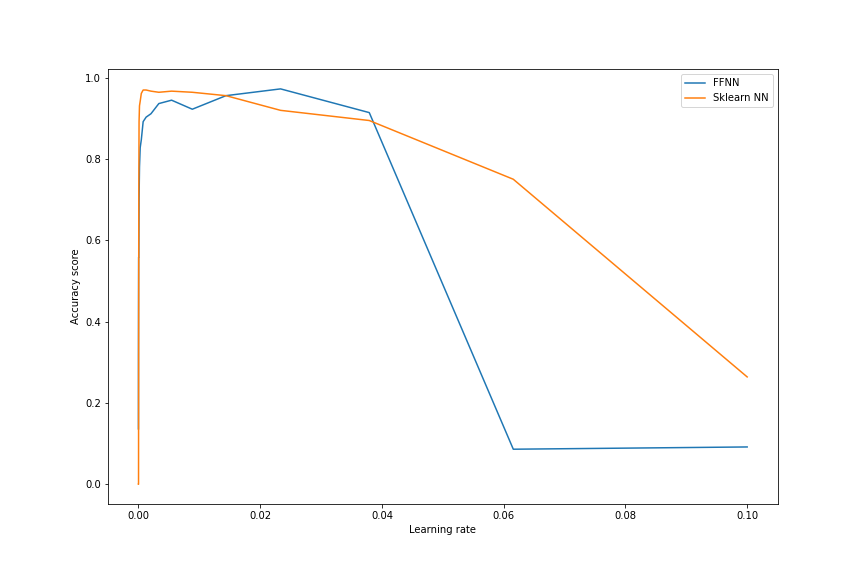
\includegraphics[trim=75 0 0 0, scale=0.2]{Partd-2}
	\caption{Accuracy score over a range of 20 learning rates from log(-5) to log(-1)}\label{figure}
	
\end{figure}

\begin{figure}[!ht]
	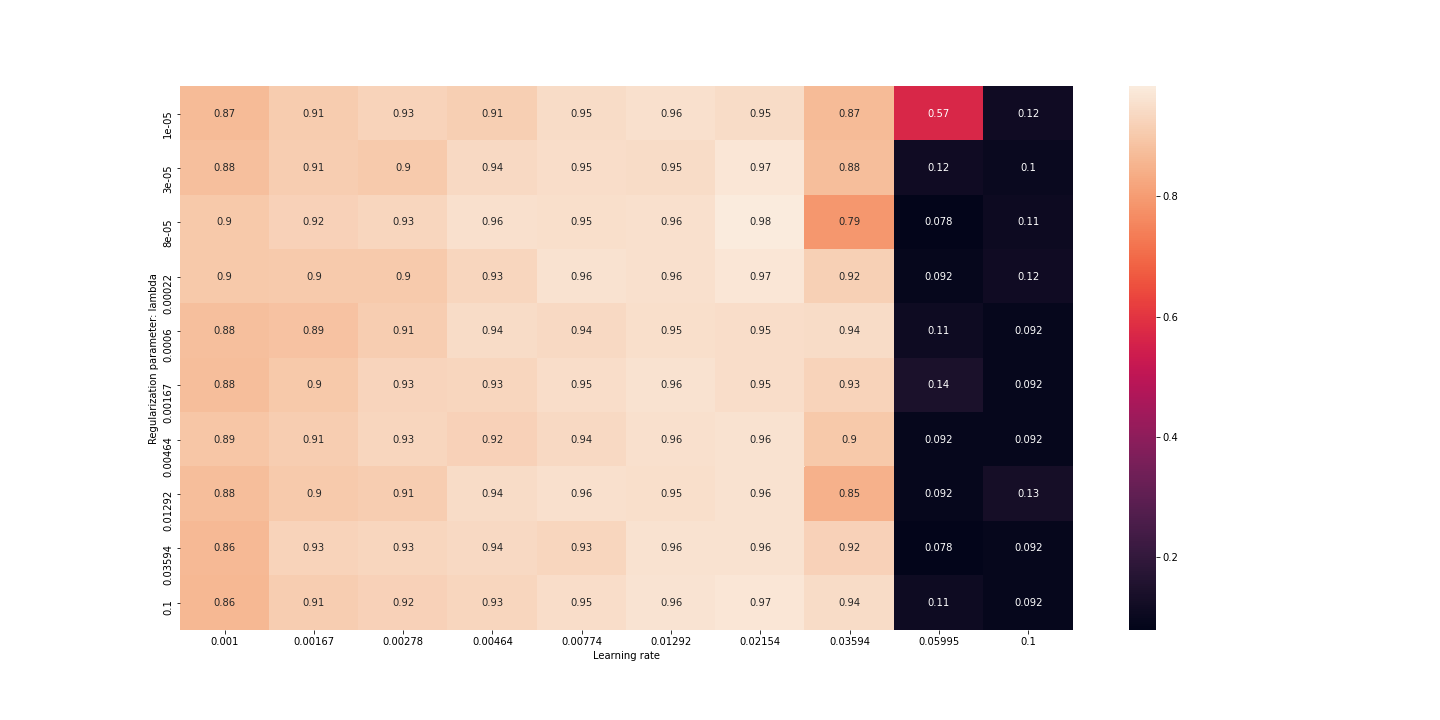
\includegraphics[trim=250 0 0 0, scale=0.2]{Partd-3}
	\caption{Accuracy score for the neural network over learning rates and regularization parameter lambda.}\label{figure}	
\end{figure}
\begin{figure}[!ht]
	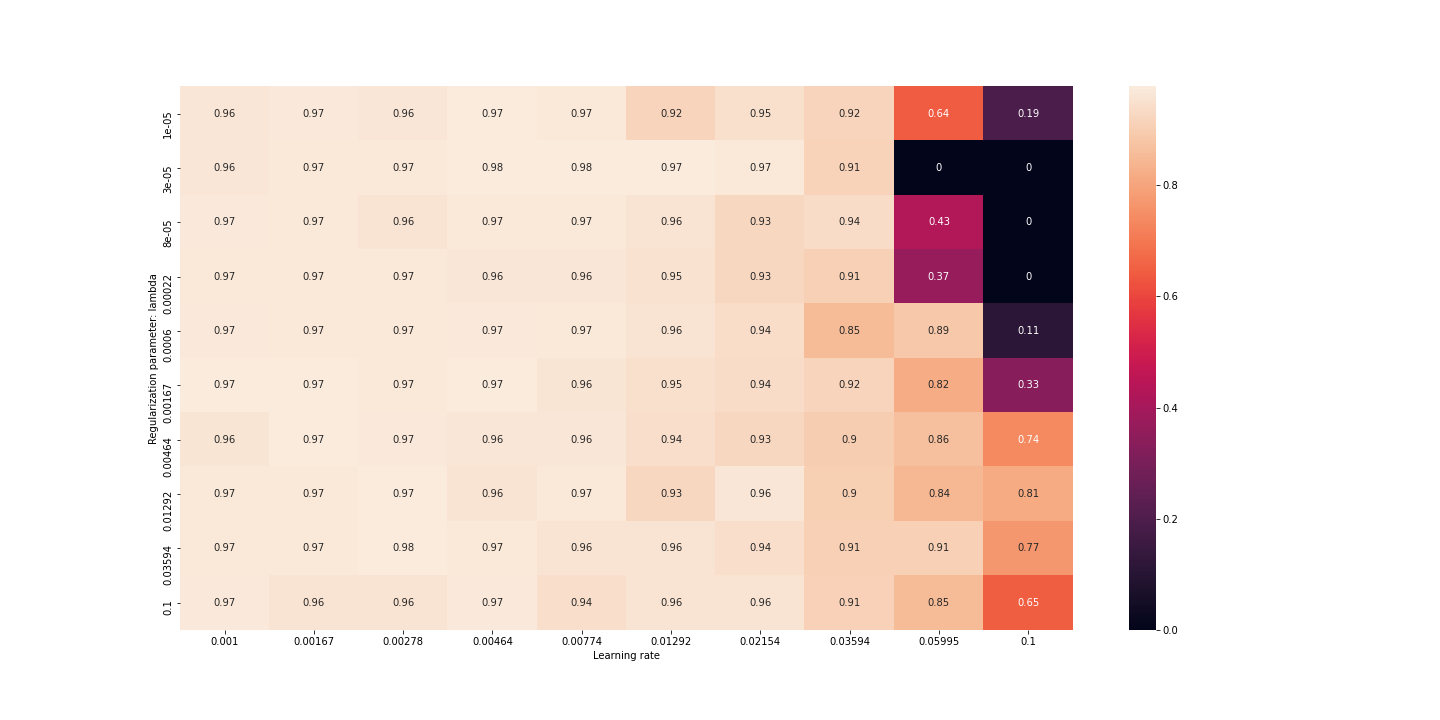
\includegraphics[trim=250 0 0 0, scale=0.2]{Partd-4}
	\caption{Accuracy score for the Scikit-learn neural network over learning rates and regularization parameter lambda. }\label{figure}	
\end{figure}
\begin{figure}[!ht]
	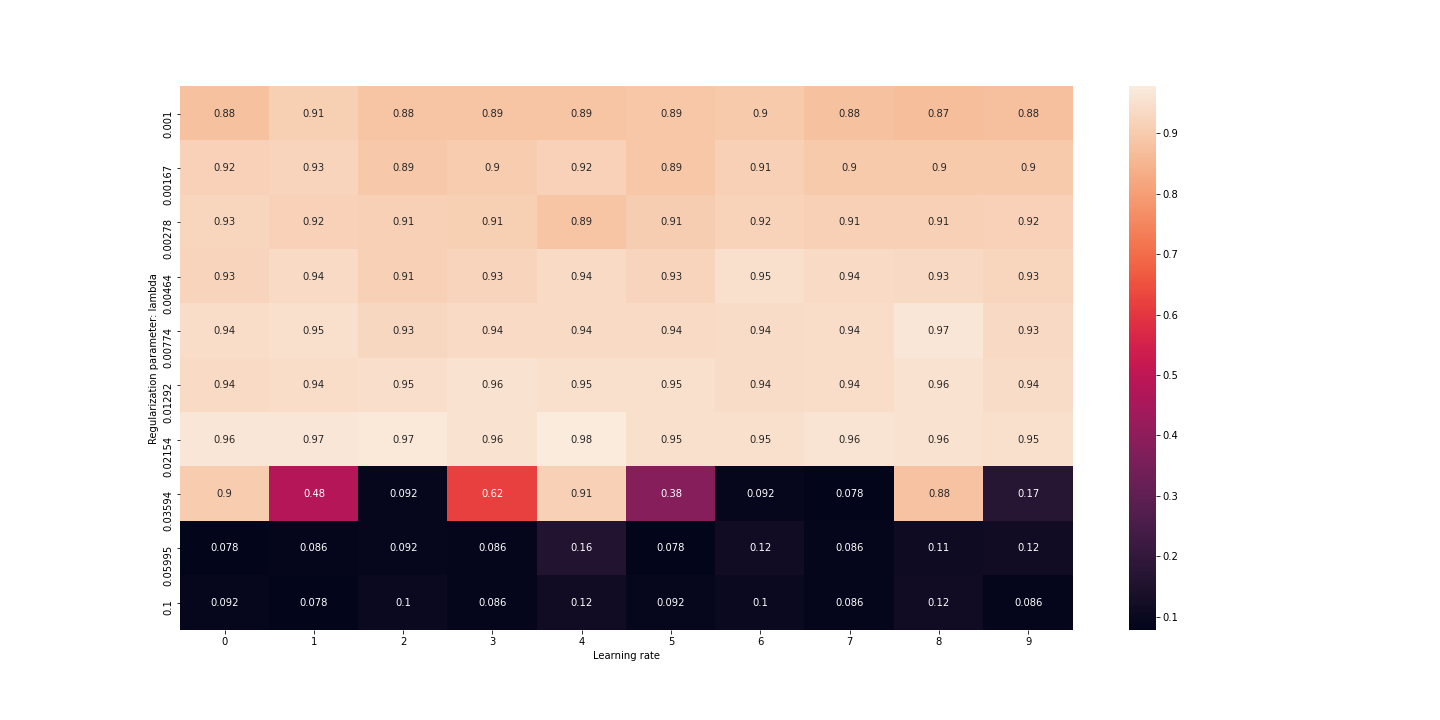
\includegraphics[trim=250 0 0 0, scale=0.2]{Partd-5}
	\caption{Accuracy score for the neural network with two hidden layers with 100 nodes each over learning rates and regularization parameter lambda. }\label{figure}	
\end{figure}

\begin{figure}
	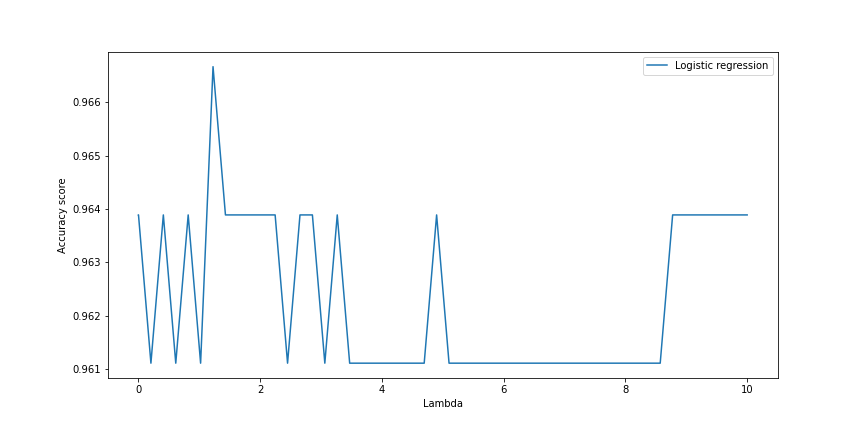
\includegraphics[scale=0.3]{Parte-1}
	\caption{Accuracy score of logistic regression on the MNIST dataset plotted against a range of regularization parameters.}
\end{figure}

\section{Discussion}

The stochastic gradient descent method was used to train models on the Franke function for linear regression and Ridge regression with a regularization parameter lambda.The experiment was done over a range of learning rates for all three models.  The linear regression seem not to have a very strong dependence on the learning rate, atleast not the range of rates chosen here. This is quite strange as the Ridge regression and Scikit-learns SGD Regression seems to be reacting to a changing learning rate, leading me to suspect some flaw in the code. 

The ridge regression have been trained over a range of lambdas from 0.1 to 1 and learning rates ranging from log(-5) to log(-0.02). The ridge model seems to be sensitive to the learning rate and seems to be converging on a MSE score of 0.87 at the higher end of the learning rate range. This is quite close to the MSE score produced by the Scikit-learn model. But the low error score is at the lower range of the learning rates for Scikit-learn whiles my ridge model has it low scores at the high end. This is quite unexpected and could be the result of some flaw in the code or misunderstanding in implementing the SGDRegressor. 

Next I implemented a Forward-feed neural network for the Franke function with 100 data points. The network is tested together with OLS regression, ridge regression and an Scikit-learn MLPRegressor implementation. The model was tested using bootstrap with 50 iterations and analysed with a range of 0 to 21 polynomial degrees. The two neural networks was implemented using one hidden layer of 50 nodes and the sigmoid activation function. For regression no activation function is used on the output layer. Number of epochs was 50. 

Figure 5 show the MSE score for a selection of the polynomial degrees and learning rates, here with no regularization. At the lower degrees of complexity the OLS method seems to be performing fairly well while my implementation of the neural network is performing quite worse and does not match the Scikit-learn implementation which also performs well. But as complexity increases the OLS MSE seems to blow up while the neural networks remain quite stable. Looking at Figure 6 one sees the mean of the MSE over all polynomial degrees plotted against the learning rate. There is an distinct difference in behavior for the two implementations which I had expected to perform quite similar. The learning rate of 0.1  seems to be close to the optimal for both models and will be used in the analysis of regularization of the models. 

Regularization parameter is implemented for a range of log(-2) to log(1) for both ridge regression and the neural networks. The architecture of the networks are the same as before. The ridge regression is performing quite well over the complexity of the model, see Figure 7, suggesting success in avoiding over-fitting of the model. Ridge seems to be performing better towards the higher end of lambda values, but overall remaining quite stable. 

The implementation of my neural network seems to be performing quite worse looking at Figure 8. A general higher MSE score overall. The models seems to be quite stable and does not blow up at higher polynomial degrees as did the OLS regression, suggesting it does not over-fit. But it does perform quite worse than the MLPRegression from Scikit-learn which is more in line with the performance of the ridge regression. Figure 10 shows three different plots for different values of lambda, plotting the log(MSE) over the polynomial degrees. It clearly shows the OLS regression blowing up  while the ridge and neural networks remaining stable across lambda values. 

Looking to other activation functions for the neural networks hidden layer I implemented the RELU and leaky RELU functions for the hidden layer. Looking at Figure 12 we see quite high MSE scores for the neural network implementation and it seems to be blowing up with the polynomial degree. The relative difference between the RELU and leaky RELU seems to be small. The scikit-learn implementation is performing alot better, but it also seems to be blowing up at higher polynomial degrees, as can be seen in figure 11. 

\subsection{Classification}
The neural network will be implemented for classification together with an MLPClassifier from Scikit-learn. Training on the MNIST dataset, with a training set of 1437 pictures, each with a total of 64 pixels as features. The network is first trained with one hidden layer of 100 nodes at 100 epochs and batch size of 50. Using the sigmoid function for activation in the hidden layer and softmax for the output layer. Network is trainer over 20 different learning rates from log(-5) to log(-1). Figure 13 shows the accuracy score of my network and the Scikit-learn implementation. Both models reaches a max score of about $94 \%$ at a learning rate from about 0.01 to 0.025. Before both models suffers in performance as the learning rate increases. The Sklearn models performs a bit better at the higher learning rates. 

Using regularization improves the models somewhat, but not a great deal. My neural network reaches a max accuracy score of 96.67 \% while the Scikit-learn model reaches 97.2 \%. Both models seems to be more dependent on learning rate than regularization. The Scikit-learn model holds up better at higher learning rates and seems to favor higher lambdas at the high end of learning rates. 

Trying out adding an additional layer to the network, this one also with 100 layers we see the heatmap flip. The models becomes sensitive to regularization and performs worse at higher lambdas. This was quite unexpected and I do not know how to explain this.    

Training a logistic regression on different values for regularization produces scores that are quite similar to the neural networks. The model seems quite stable across regularization parameters. 

\section{Conclusion}
In the regression experiments the neural networks seems to comparable to the Ridge regression, being stable across an increase in the complexity of the model. Even without regularization the neural networks have a stable profile. My own network seems to perform a bit worse than the Scikit-learn implementation, a bit disappointing, although being stable. 

On the classification part my neural network seem to perform quit well, able to reach accuracy score of 97 \% and here my network seems to be able to keep up with the Scikit-learn implementation. But having some faster decline in performance when learning rate increases. I conclude that regularization did not have a big inpact on the classification models. Learning rate was a far bigger influence with one later. Adding a second layer flipped that and made regularization matter more, this was an interesting discovery. 



\section*{References}  % the asterisk (*) after \section makes the section numbering go away
[1] Aurelien Geron - Hands-on Machine Learning with Scikit-Learn, Keras \& TensorFlow: Page 122, equation 4-7 : Gradient descent step

\end{document}
